%\documentclass[tikz,a4paper]{article} % стандартный документ
\documentclass[tikz,a4paper]{scrartcl} % документ с подзаголовком
\setkomafont{disposition}{\normalfont\bfseries} % шрифт (под)заголовков

\usepackage[russian]{babel} % русский текст
\usepackage[utf8]{inputenc} % русский в кодировке UTF8
\usepackage{amssymb,amsfonts,amsthm,amsmath} % математика
\usepackage{graphicx,graphics} % рисунки
\usepackage{cite} % расширенный тип цитирования
\usepackage[square,sort,comma,numbers]{natbib} % расширенный тип библиографии
\usepackage{authblk} % форматирование имeн автора и аффилиации
\usepackage{pgfplots} % графики функций

\usepackage{tikz} % диаграммы
\usetikzlibrary{positioning,shapes,arrows,matrix}
\usetikzlibrary{decorations.pathmorphing,backgrounds,fit,petri}
\usetikzlibrary{calc,intersections,through,backgrounds}

\usepackage{geometry} % установка полей документа
\geometry{left=3cm,right=3cm,top=3cm,bottom=3cm}

\begin{document}

\title{Алгоритм эффективной генерации цепочек на сетке}
\subtitle{/техническое задание/}
\author{Э.~С.~Фомин}
\date{} % не печатать дату генерации документа
\maketitle
\large % размер фонта всего документа


\section*{Постановка задачи}
\textit{Задача}. Дана цепь длины $L$, где $L$ находится в диапазоне $[128, 1024]$ элементов. Цепь разбита на $N$ последовательных участков длины $L_i$, $\sum_i^N L_i = L$. Каждый участок последовательно пронумерован. Цепь складывается в пространстве в некоторую компактную\footnote{Смысл понятия <<компактность цепи>> определяется далее.} структуру. Полученная структура исследуется на контакты ее участков с получением таблицы контактов. Таблица контактов является двумерной, и содержит число контактов для любой пары участков. Необходимо, имея только таблицу контактов, восстановить структуру цепи. Предполагается, что задача имеет большое множество решений, потому целью задания является эффективная генерация множества решений, удовлетворяющих заданным ограниченим по контактам.

Требуется реализовать несколько вариантов задачи, отличающихся пространством поиска, типом сетки и таблицы контактов.
\begin{itemize}
\item пространство поиска является двумерным (сетка на плоскости) и трехмерным (сетка в объеме),
\item сетка должна быть задана как BFM сетка (bond fluctuation model) \cite{BMF1994}, поскольку построение цепи именно по такому типу сетки обеспечивает большую гладкость,\footnote {Экспериментальные версии кода могут использовать равномерные сетки.}
\item таблица контактов должна рассматриваться как таблица с целыми, так и с булевыми значениям, $U_{ij} = 0 \Rightarrow false$ и $U_{ij} > 0 \Rightarrow true$.
\end{itemize}

\section*{Предполагаемый вариант решения}
Эффективность простого перебора с возвратами неприемлима для решения задачи с заданной длиной цепочки, поскольку его вычислительная сложность оценивается как $3^L$ для равномерной сетки на плоскости, или $\geq 5^L$ для сетки в пространстве. Потому \textit{метод полного перебора должен быть исключен}\footnote{Метод полного перебора может и должен использоваться для тестирования более быстрых, но не гарантирующих нахождение всех решений, эмпирических или прочих методов.}. Предлагаемый вариант решения основан на генерации цепочек вариантом метода Монте-Карло, в котором вероятность того или иного направления роста цепи зависит как и от локального окружения точки (число соседей), так и расстояния до точки контакта. Предполагается, что корректный подбор функции оценки для выбора направления роста цепи позволит с большой вероятностью выполнять генерацию цепей, удовлетворяющих как требованиям компактности, так и ограниченим по контактам.

\subsection*{Как выбирать направление роста цепи}
Направление роста цепи зависит от многих факторов, причем наиболее существенными из них являются:
\begin{enumerate}
\item модель цепи, которая отражает основные особенности моделируемого объекта (жесткость к изгибу, жесткость к кручению, склонность к изломам, однородность жесткости вдоль цепи), 
\item модель укладки цепи (компактность, разреженность, фрагментарность,  кластеризация, наличие мотивов укладки и прочее), 
\item модель проницаемости (<<жесткие>> и <<мягкие>> стерические ограничения, внешние ограничения в пространстве), 
\item модель контактов с участками уже построенной цепи,
\item модель потенциалов,
\item модель учета энтропийного фактора.
\end{enumerate}
И все эти факторы должны быть корректно, то есть, как минимум в первом приближении точности, заложены в функцию, которая выбирает направление дальнейшего роста цепи (<<функция выбора>>). Заметим, что методологически проще выбирать разные функции выбора для разных моделей цепи и разных типов укладки. И наоборот, прочие требования - способ избегания стерических затруднений, обеспечения контактов и учета энтропии - должны учитываться в любой функции выбора. 

\begin{quote} \textit{Отступление для понимания}. 

Процесс выбора неформально может быть описан следующим образом. Допустим, мы имеем цепь, жесткую к изгибам и мягкую к кручению, однородную и не имеющую склонности к изломам (это наиболее естественный вариант цепи для предметной области). Это означает, что каждый следующий сегмент цепи $i$ по своему направлению достаточно мало отличается от направления предыдущего сегмента $i-1$ (жесткость к изгибам). При этом двугранный угол между плоскостями, образуемыми сегментами ($i-1$, $i$) и ($i$, $i+1$) меняется хаотическим образом вдоль цепи (свободно крутящаяся цепь). Вопрос. Как для такой цепи работает функция выбора?

Функция выбора должна учесть, что точки сетки, которые находятся в направлении последнего построенного сегмента цепи $\bold r_{i,i+1}$, должны иметь приоритет перед точками в стороне или ведущими цепь в обратном направлении. Причем выбор любой точки из тех, что находятся на окружности вокруг вектора $\bold r_{i,i+1}$, должен быть равновероятен (цепь является свободно крутящейся). 

Расставив вероятности выбора точек, зависящие от модели цепи, функция выбора должна учесть модели укладки, и соответствено скорректировать вероятности точек. Например, для модели плотной упаковки вероятности точек, которые локализованы рядом с уже построенной цепью должны быть выше, а для точек, рядом с которыми нет ни одной занятой точки, вероятность выбора должна быть близка к нулю.

Учет стерических затруднений выполняется наиболее просто, вероятности выбора точек, которые уже заняты цепью, обнуляются.

И последнее. Допустим, что в цепи есть контакт $AB$, и элемент цепи $A$ уже построен, а элемент $B$ еще нет. Функция выбора в этом случае должна повышать приоритет у точек, которые находятся в сторону элемента $A$, чтобы в конце концов свести точку цепи $B$ к $A$.

\end{quote}

Разберем факторы, влияющие на рост цепи подробно.
\subsubsection*{Модели цепи}
Требуется реализовать две модели цепи - однородную и неоднородную (в приближении <<средней жесткости>>). Обе модели являются параметрическими, и учитывают жесткость по сгибу и кручению параметрами $k_b$ и $k_t$, соответственно. 

\textit{Однородная модель} характеризуется тем, что параметры жесткости $k_b$ и $k_t$ вдоль цепи не меняются. Также в однородной модели нет склоности к изломам цепи, и изломы игнорируются.

\textit{Неоднородная модель} характеризуется тем, что вдоль цепи ее жесткость переменна. Причиной, которая приводит к изменениям жесткости, можно считать изменение состояния элементов цепи. Таким образом, в модели элементы цепи имеют атрибут, называемый состоянием. Число возможных состояний элементов $N_s$ фиксировано, и в предметной области это число ограничено небольшим значением, $N_s \lesssim 10$. Состояние любого элемента цепи определено, и оно  задается во входных данных. Для каждого состояния определены свои значения жесткости $k_b$ и $k_t$. Благодаря тому, что в цепи есть участки с нулевой жесткостью, в модели возможны резкие изломы цепи\footnote{Участок с нулевой жесткостью к изгибу может приводить, а может и не приводить, к излому цепи. Нулевая жесткость означает только одно - равновероятность выбора угла изгиба. Наиболее реальна ситуация, когда цепь имеет резкий излом с фиксированным углом изгиба. Фиксированный угол означает высокую жесткость $k_b \neq 0$ при равновесном угле сгиба отличном от 0. Итого, аттрибут <<состояние>>, чтобы уметь учитывать такую ситуацию должен включать не только параметр жесткости $k_b$, но и параметр равновесного угла $\theta$.}.

\subsubsection*{Модели упаковки}
Требуется реализовать модель плотной (компактной) упаковки. Плотная упаковка означает, что цепь на сетке размещается таким образом, что свободных ячеек внутри области, охваченной цепью, достаточно мало. Плотность упаковки может меняться в разных точках сетки $\bold r$ и характеризуется параметром $\rho(\bold r)$, который вычисляется следующим образом. Некоторая точка сетки откружается кубом с длиной ребра $l$, и рассчитывается $n_a(l)$ - полное число ячеек в кубе, $n_a(l) \sim l^3$, и $n_f(l)$ - число занятых ячеек в кубе. Локальная плотность упаковки в точке $\bold r$ определяется как 
\begin{equation}
\rho(\bold r) = \lim_{l\rightarrow 0} \frac{n_f(l)}{n_a(l)} 
\label{eq:local_density}
\end{equation}
Полная усредненная плотность упаковки вычисляется как среднее значение плотности по всем точкам, через которые проходит цепь, 
\begin{equation}
\rho = \frac{\sum \rho(\bold r)\delta_c(\bold r)}{\sum \delta_c(\bold r)} = \frac{1}{L} \sum_{\bold r} \rho(\bold r)\delta_c(\bold r)
\label{eq:density}
\end{equation}
В последней формуле выполняется суммирование по всем точкам $\bold r$ сетки.  Функция $\delta_c(\bold r)$ характеризует захват цепью $c$ точки сетки $\bold r$, и она равна 1 или 0 в зависимости от того, захвачена или нет точка. 

\begin{figure}[h]
\center{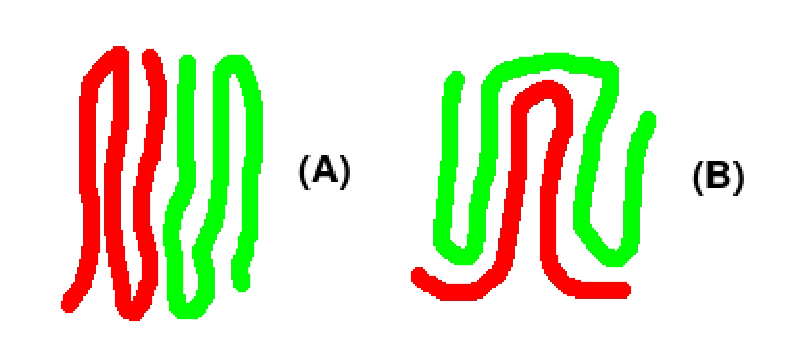
\includegraphics[width=1\linewidth]{images/fold.eps}}
\caption{(A) Тип упаковки (спутывание близких нитей), генерируемый функцией оценки. (B) Тип упаковки (спутывание далеких нитей), теряемый функцией оценки.}
\label{pic:fold}
\end{figure}
 
Формулы (\ref{eq:local_density}, \ref{eq:density}) позволяют вычислять плотность, вопрос заключается в том, как генерировать цепочки с учетом плотности упаковки $\rho(\bold r)$. Проблема заключается в том, что если генерация цепи выполняется последовательно, то есть поначалу цепь строится в пустом пространстве, которое постепенно заполняется, то \textit{внешние условия при построения цепи постоянно меняются}. Как результат, при заданной функции оценки плотности, цепь сразу начнет складываться таким образом, чтобы обеспечить нужную плотность упаковки. А это нарушение требований на корректный учет энтропийного фактора, поскольку цепи типа A получают преимущество над цепями типа B (см. рис.\ref{pic:fold}). Заметим, что случай A включает структуры, в которых плотность упаковки обеспечивается перепутыванием близких в пространстве нитей, а случай B - перепутыванием нитей, которые далеко разнесены в пространстве.

\subsubsection*{Модели проницаемости}
\textit{<<Жесткие>> стерические ограничения}. Требуется реализовать модель <<жестких>> стерических ограничений для полноразмерной задачи. Жесткие ограничения означают, что одна и та же область пространства не может быть захвачена несколькими элементами цепи.

\textit{<<Мягкие>> стерические ограничения}. Для грубозернистых моделей, где размер элемента сетки увеличен и элементы цепи объединены в более масштабные объекты, необходимо использовать модель <<мягких>> стерических ограничений. Мягкие ограничения означают, что одна и та же ячейка сетки может быть захвачена несколькими кусками цепи. Сколько раз одна и та же ячейка может быть захвачена зависит от степени изменения масштаба модели.

\begin{quote} \textit{Отступление для понимания}. 
Допустим, мы строим цепь на сетке плоскости. Пусть она разграфлена как шахматная доска (от a1 до h8). Пусть цепь имеет контакт около центра доски, например, проходит в прямом направлении по клеткам \{c3,c4\} и в обратном направлении по \{d4,d3\}. Перейдем к крупнозернистой модели, в которой клетки доски объединены \{a1, a2, b1, b2\} в одну клетку A1, \{a3, a4, b3, b4\} в одну клетку A2 и т.д., и любые два элемента цепи также рассматриваются как единые элементы. Теперь на большой сетке новая клетка B2, в которую попадают старые клетки \{с3, с4, d3, d4\}, может быть захвачена только одним элементом новой цепи. Но ведь ранее через это место проходило два куска цепи сразу. Итого, на грубозернистой сетке мы потеряем одно из возможных решений, либо произойдет сильное искажение решения, поскольку один из кусков цепи будет смещен в другие области решений. Таким образом, модель <<жестких>> стерических ограничений вносит сильные искажения в решение. 

Для ликвидации подобного рода дефектов необходимо использовать модель, в которой одна и та же клетка может быть захвачена несколько раз. В используемом примере, очевидно, что клетка B2 может быть захвачена не более 2-х раз.
\end{quote}

Итак, сколько раз может быть захвачена одна и та же клетка в грубозернистой модели?  Ответ на этот вопрос зависит плотности упаковки цепи. 

\textit{Степень захвата для компактной упаковки, $\rho = 1$}. Для компактной упаковки цепи получить ответ на заданный вопрос достаточно просто. Допустим, мы увеличили масштаб в $m$ раз, то есть одна <<новая>> клетка занимает то же пространство, что и $m^d$ <<старых>> клеток, где $d$ - размерность пространства. Поскольку в плотной упаковке через данную область пространства ранее проходило $n = V_{cell}/V_{chain} = m^d/m = m^{d-1}$ кусков цепи, где $V_{cell}$ - объем <<новой>> клетки,$V_{chain}$ - минимальное число элементов <<старой>> цепи, необходимых, чтобы полностью пересечь <<новую>> клетку, то такова же и должны быть разрешенная кратность захвата клетки в грубозернистой модели, то есть $n = m^{d-1}$.

\textit{Степень захвата для разреженных упаковок, $\rho < 1$}. Если упаковка разрежена, $\rho < 1$, то число фрагментов пересекающих объем пространства, равный <<новой>> клетке, уменьшается. Оно может быть оценено как $n = \rho m^{d-1}$, причем такова же будет возможная кратность захвата.

\textit{Есть ли выгода от грубозернистых моделей?} На первый взгляд кажется, что никакой выгоды от перехода к грубозернистой сетке нет. Число подобъектов для моделирования снижается (это плюс в эффективности), но кратность возможного захвата ЛЮБОЙ клетки (а не только той, где происходит касание) пропорционально увеличивается с увеличением числа возможных вариантов размещения (что минус в эффективности). Тем не менее выгода есть. 

Чтобы понять, что она существует, достаточно рассмотреть предельный случай - размер ячейки увеличен в $L$ раз, где $L$ - длина цепочки, и цепь является одним объектом. В этом предельном случае число вариантов решения равно 1 (весь объект помещается в одну клетку). В старой сетке число вариантов размещения $3^L$ и более. То есть, выгода заключается в том, что множество близких траекторий прохождения цепи на мелкозернистом уровне объединяются в единую траекторию на грубозернистом уровне.

\subsubsection*{Модель контактов}
Поскольку длина контактирующих участков цепи больше 1, то контакт участков может произойти в любом месте. Если длина участка $i$ равна $L_i$, а длина другого участка $j$ равна $L_j$, то число вариантов состыковки этих участков цепи равно $n_{ij} = L_i L_j$, и все эти варианты принадлежат одному и тому же контакту. Множественность вариантов состыковки требует учета энтропийного фактора (см. ниже).

Примитивные модели контакта, такие как контакт по центрам участков, или контакт по началам участков, могут рассматриваться только в первоначальных пробных реализациях. 

\subsubsection*{Модель потенциалов}
Вероятность выбора направления цепи может регулироваться модельными потенциалами, то есть в рассмотрение вводится понятие энергии $E(\Gamma(\bold r))$ конфигурации цепи $\Gamma(\bold r)$. Конфигурация цепи $\Gamma(\bold r)$ определяется как совокупность занятых в пространстве ячеек с учетом типа элемента цепи в той или иной ячейке. При введении потенциалов, приоритет в направлении роста цепи получают те ячейки, размещение цепи в которых минимизирует полную энергию $E(\Gamma(\bold r))$ конфигурации.\footnote{Предполагается необходимость введения модельных потенциалов для обеспечения группировки фрагментов цепи, находящимся в одном состоянии.} 

\begin{center} 
to be continued...
\end{center}

\subsubsection*{Учет энтропии}
Везде, где существует некоторая зависимость свойств объекта от числа возможных размещений (или состояний) ее элементов, возникает энтропия. Энтропия $S$ определяется как логарифм от числа вариантов размещения, $S = \ln W$. Именно большое число вариантов размещения не позволяет реализовываться упорядоченным структурам (их число и, следовательно, вероятность появления по сравнению с неупорядоченными структурами чрезвычайно мала\footnote{За исключением случаев, когда реализация упорядоченного состояния существенно энергетически выгодней, нежели неупорядоченного.}). Следовательно, при генерации различных размещений цепи на сетке необходимо обеспечить низкую вероятность появления упорядоченных состояний.

\begin{quote} \textit{Примером неудачной реализации}, которая игнорирует энтропийный фактор, является генерация кольцевой цепочки следующим образом. Цепочка стартует от некоторой точки и продвигается случайным образом до тех пор, пока сохраняется достаточное число путей возврата\footnote{Возможно эффективно отслеживать самый короткий путь возврата используя технику динамического программирования.} к исходной точке. Как только путь возврата остается единственным, цепочка замыкается (почти по прямой линии) с началом. Очевидно, что такая генерация дает большое число частично упорядоченных траекторий, что должно быть запрещено для моделей, которые описывают реальный мир.
\end{quote}

\textit{Учет энтропийного фактора для моделей цепи} выполняется следующим образом. Допустим, что цепь имеет жесткость к сгибу $k_b$. С какой вероятностью необходимо выбирать угол сгиба между звеньями цепи? Естественным выбором является выбор такой вероятности, чтобы полученное распределение по углам имело Больцмановское распределение\footnote{Является ли это распределение Больцмановским? Скорее всего, это самая разумная гипотеза, и большое число физических объектов реального мира демонстрируют это поведение. Можно проверить это на реальном объекте? Да, если обработать ряд баз данных по пространственному строению белков.}, то есть 
\[ p(\theta) \sim \exp \left(-\frac{k_b \theta^2}{2kT} \right)  \]
где $k$ - константа Больцмана, $T$ - абсолютная температура.

\textit{Учет энтропийного фактора при наличии потенциалов} выполняется так же с помощью Больцмановского распределения.
\[ p(\Gamma(\bold r)) \sim \exp\left(-\frac{E(\Gamma(\bold r))}{kT}\right)  \]

\textit{Учет энтропийного фактора для моделей контакта}. Казалось бы, что два участка $i$ и $j$ с длинами $L_i$ и $L_j$ могут контактировать в любом своем месте с равной вероятностью, то есть вероятность любой состыковки участков равна $p = 1 / L_i L_j$. Тем не менее, это не всегда так. 
\begin{quote} Как контрпример можно рассмотреть жесткую цепь с участками, пересекающимися под прямым углом в центре координат (0,0). Поскольку цепь жесткая, то вариантов для нее достаточно изогнуться и избежать пересечения в точке (0,0) весьма немного. Таким образом, вероятностное распределение по вариантам стыковок будет нормальным Гаусовским распределением с максимумом в (0,0).
\end{quote}

\textit{Число вариантов для заданной длины.} Пусть два участка длиной $L_1$ и $L_2$ контактируют, причем общая длина цепи между ними равна $l_{12}$. Участки могут пересекаться любым образом, и общая длина между кольцевого участка цепи, задаваемого пересечением, находится в диапазоне от $L_{min} = l_{12}$ до $L_{max} = L_1 + l_{12} + L_2$. Вопрос. Сколько вариантов стыковок дают заданную длину кольцевого участка $l$? Ответ. Длину равную $L_{min}$ или $L_{max}$ дает только один вариант. Промежуточные длины задаются большим числом вариантов. 

\[ n(l) = \begin{cases} 
0 			&\mbox{if } l < L_{min} \\ 
l - L_{min}	&\mbox{if } L_{min} \leq l \leq L_{min} + m \\ 
m			&\mbox{if } L_{min} + m < l < L_{max} - m \\ 
L_{max} - l 	&\mbox{if } L_{max} - m \leq l \leq L_{max}  \\
0 			&\mbox{if } l > L_{max} 
\end{cases} \]
где $m = \min(L_1, L2)$. То есть, образуется область длин от $l-L_{min}$ до $L_{max}-l$ в которой число вариантов константно и равно $m$. У нас нет резкого пика, и нет предпочитаемых длин. Это означает непригодность методов генерации цепей, основанных на некоторых усредненных длинах колец, образуемых стыковками (например, по центрам участков) (см. ниже). Если $L_1 = L_2$, то найденная область длин вырождается в точку со значением $(L_1 + L_2)/2$.

Тем не менее, наличие пусть и слабого подъема числа состояний для промежуточной длины кольца позволяет дать рекомендации по построению алгоритма. Начинать нужно для средней точки $(L_{min} + L_{max})/2$, где число вариантов максимально и равно $m$, а зетем переходить к краям интервала [$L_{min}$, $L_{max}$].

\section*{Алгоритмика}
\subsection*{Генерация множества структур кольца длины L}
Наиболее типичным случаем для построения кольца (как части цепочки) будет случай, когда кольцо нужно будет строить в некоторой относительно свободной области пространства. Остальная часть пространства будет занята ранее построенными частями цепочки. Случай, когда вся сетка в пространстве свободна, нетипичен, поскольку появляется только в начале построения.

Пусть задана некоторая свободная область на сетке и некоторая стартовая точка $A$. Необходимо построить замкнутое кольцо длины $L$, которое стартует в точке $A$, без разрывов и самопересечений проходит по свободной области сетки и возвращается в точку $A$. Цепь обладает заданной жесткостью к изгибу $k_b$ и жесткостью к кручению $k_t$. Требуется эффективный алгоритм генерации таких колец.

Основная идея алгоритма заключается в том, чтобы разделить цепь $L$ на две равные части длиной $L/2$, запустить построение обоих половинок от точки $A$, и объединять половинки цепи в конечных точках, если они попадают в одну и ту же ячейку сетки.

Алгоритм включает следующие шаги:
\begin{enumerate}
\item сгенерим и сохраним в памяти множество цепочек, стартующих от точки $A$ и проходящих по свободной области пространства без самопересечений,
\item создадим массив $B$, каждый элемент которого хранит ссылку на некоторую цепочку, упорядоченные идентификаторы двух последних точек этой цепочки и знак направления между двумя последними точками цепочки,
\item отсортируем массив $B$ по идентификаторам двух последних точек цепочек и по их направлению,
\item соединим те цепочки, которые совпадают по идентификаторам двух последних точек и противоположны по их направлению,
\item удалим цепочки с самопересечениями
\end{enumerate}

Вычислительная сложность такого алгоритма заметно меньше, чем у алгоритма генерации цепочки с полной длиной $L$ (который будем называть <<наивным>>). Сделаем оценку для самого худшего случая, когда жесткость цепи $k_b=0$, и цепочка хаотично движется во всех направлениях в пространстве с размерностью $d=3$. Будем считать, что разрешенное число направлений движения на сетке вычисляется как $n_d = 2d$, а не $n_d = 2d-1$, то есть $n_d =6$ (игнорируем направление возврата для упрощения). Имеем для каждого шага: 
\begin{enumerate}
\item Число сгенерированных цепочек равно $N = n_d^{L/2} \sim 6^{L/2}$. То есть, число операций $N_1 = N L \sim 6^{L/2} L$.
\item Размерность массива $3 N$, число операций $N_2 = 3 N \sim 6^{L/2}$.
\item Число операций сортировки $N \log N \sim 6^{L/2} L$.
\item Число ячеек, куда может попасть последняя точка цепочки $\frac{4\pi}{3}(L/2)^3 \sim L^3/2$. Предпоследняя точка попадает всегда рядом с последней, то есть число возможных пар двух последних точек цепочки равно $\frac{4\pi}{3}(L/2)^3 n_d \sim L^3$. Этому же значению равно число групп $N_g \sim L^3$, на которые разбиваются все $N$ цепочек, при этом число элементов в группе $n_g = N/N_g \sim N/ L^3$. Поскольку связываться могут только половинки цепочек, попавшие в одну группу, то полное число результирующих цепочек длины L равно $N_{sol} = n_g^2 N_g \sim (N/L^3)^2 L^3 = N^2 / L^3 \sim 6^L / L^3$.
\end{enumerate}
Поскольку <<наивный>> алгоритм генерит $n_d^L \sim 6^L$ цепочек, а предложенный алгоритм - только $6^L / L^3$ цепочек, то отношение их эффективности пропорционально $L^3$ (с учетом затрат на сортировку отношение эффективности снижается до $L^2$).

\subsection*{Генерация колец с длиной $L \in$ [$L_{min}, L_{max}$]}
Поскольку длина контактирующих участков цепи может быть больше 1, то контакт участков происходит в любом месте. Пусть длина участков $i$ и $j$ равна $L_i$ и $L_j$, и длина участка между ними равна $l$. В этом случае нужно рассматривать всевозможные длины образующегося кольца в диапазоне от $L_{min} = l_{12}$ до $L_{max} = L_i + l_{12} + L_j$. 

Алгоритм, описанный в подсекции выше, легко может быть модифицирован для обработки всех длин в диапазоне. Идея заключается в том, чтобы вместо отдельной генерации всех цепочек с длинами в заданном диапазоне, генерить цепочки максимальной длины с извлечением более коротких цепочек из уже сгенерированныйх длинных цепочек.

\begin{enumerate}
\item установим длину цепочки равную $L_{max}/2$.
\item сгенерим и сохраним в памяти множество цепочек, стартующих от точки $A$ и проходящих по свободной области пространства без самопересечений,
\item для каждой цепочки пройдем ее последние точки от $L_{max}/2$ до $L_{min}/2$ и запишем их парами соседних точек в массив $B$, добавив ссылку на цепочку, знак направления и длину цепочки от начала до записываемой пары,
\item отсортируем массив $B$ по идентификаторам пар соседних точек и по их направлению,
\item соединим те цепочки, которые совпадают по идентификаторам двух последних точек и противоположны по их направлению, при этом суммарная длина общей цепочки должна быть в нужном диапазоне,
\item удалим дублирующие цепочки, а также цепочки с самопересечениями
\end{enumerate}

Удаление дублей необходимо, чтобы не получить проблемы с нарушением энтропийного фактора\footnote{Необходимо обеспечить, чтобы число состояний с нужной длиной цепи было пропорционально выше рассчитанным соотношениям. Как?}. 

\subsection*{Сохранение памяти при генерация колец}
Случайная генерация может привести к тому, что множество цепей начинают повторяться. Если хранить все цепи, то возможно переполнение памяти. Простой трюк может избежать хранения любых цепей с перегенерацией их при необходимости.
\begin{itemize}
\item перед запуском генерации новой цепи записываем seed случайного генератора,
\item после получения цепи записываем необходимые параметры полученной цепи (например, координаты двух последних точек цепи, используемых для сшивки половинок) вместе со значением seed,
\item данные по цепи сбрасываем для избежания переполнения памяти,
\item после набора представительного ансамбля цепей (нахождения сцепляемых половинок цепи или решения прочих задач), и в случае необходимости иметь данные по конфигурации цепей, мы перегенерируем нужные цепи заново через установку у генератора сохраненных ранее seeds.
\end{itemize}

\subsection*{Общий алгоритм}
Aлгоритм генерации полной цепи работает при ограничениях на модель укладки (модель контактов). Есть весомые доводы на то, что укладка обладает следующим свойством. Для любых двух точек цепи A и B, которые контактируют друг с другом в пространстве, не существует какой либо точки C, локализованной на цепи между точками A и B, которая бы образовывала некий контакт с какой либо прочей точкой D. То есть, любое кольцо, которое образуется контактом не содержит внутри себя других колец, и разные кольца не сцепляются друг с другом (см.рис.\ref{pic:connects}).

\begin{figure}[h]
\center{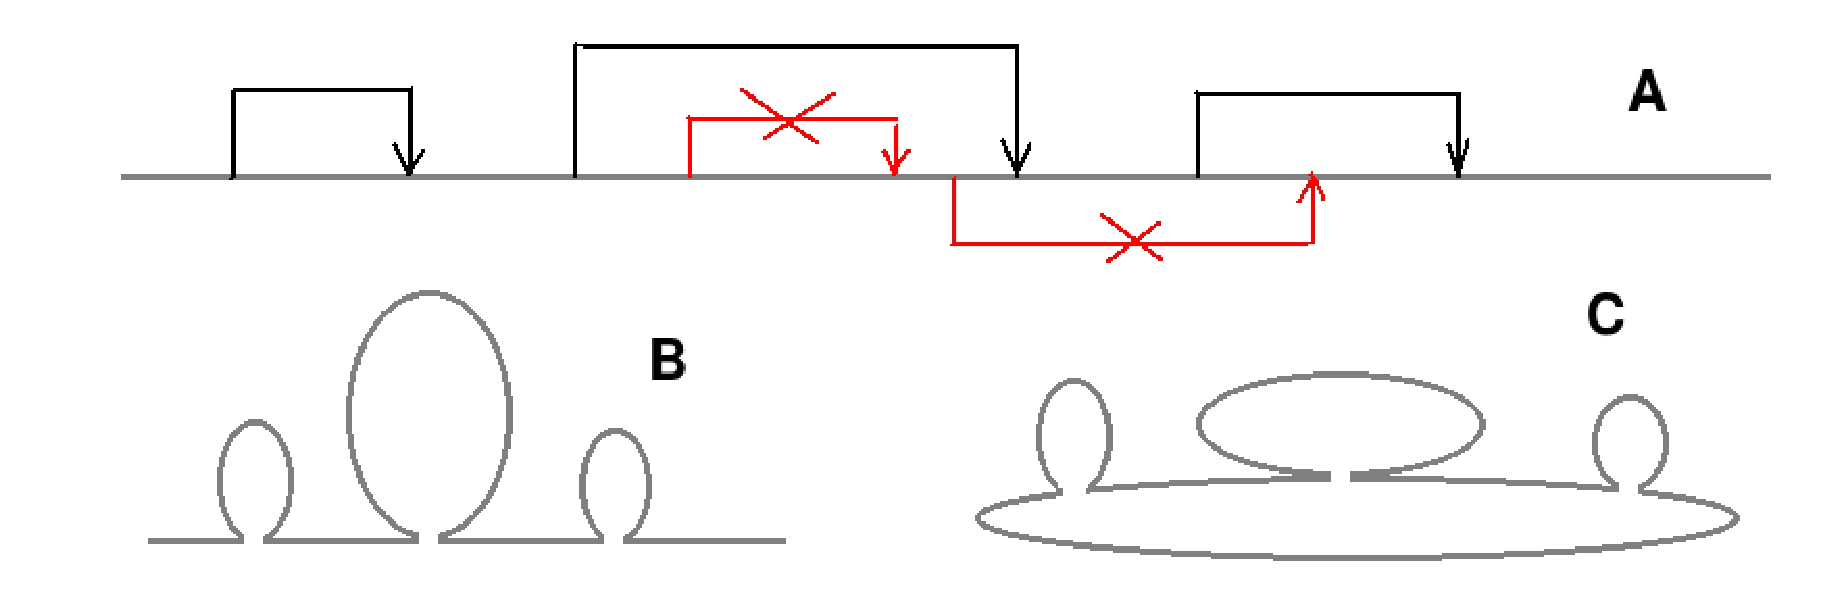
\includegraphics[width=1\linewidth]{images/connects.eps}}
\caption{(A) Наиболее характерное расположение коннектов в цепи (вложенные и сцепленные циклы, помеченные красным, отсутствуют в модели укладки). Пространственное расположение линейной цепи (B) и замкнутой цепи (C).}
\label{pic:connects}
\end{figure}

Для модели цепи, которая удовлетворяет такой укладке, алгоритм построения легко строится над алгоритмом генерации одиночного кольца, который описан выше. Расмотрим случай замкнутой цепи. Алгоритм включает следующие шаги:
\begin{itemize}
\item Генерация наибольшего по размеру кольца (см.рис.\ref{pic:connects}c).
\item Переход к точке контакта и генерация кольца от этой точки.
\item Повторение предыдущего шага по всем точкам контактов.
\end{itemize}
Если вычислительная сложность генерации одного кольца длины $L$ равна $6^L/L^2$, то вычислительная сложность полного алгоритма будет 
\[ N_{oper} \sim \prod_i \frac{6^{L_i}}{L_i^2} \]
где индекс $i$ пробегает по всем контактам.

\textit{Какое кольцо предпочтительней, чтобы быть стартовым в генерации?} Чем большая часть объекта сгенерирована, тем меньше комбинаций образуется при генерации остальных колец. Итого, выгодней, чтобы самые длинные кольца генерировались последними. Как это сделать?

\begin{thebibliography}{99}
\bibitem{BMF1994} http://en.wikipedia.org/wiki/Bond\_fluctuation\_model
\end{thebibliography}

\end{document}
